\documentclass[a4paper, 10pt, final, garamond]{book}
\usepackage{cours-preambule}
\usepackage[french]{babel}

\raggedbottom

\makeatletter
\renewcommand{\@chapapp}{Thermodynamique -- chapitre}
\makeatother

\begin{document}
\setcounter{chapter}{3}

\chapter{TD~: Changements d'\'etats}

\section{Isothermes d'\textsc{Andrews}}

\begin{minipage}[t]{.60\linewidth}
  La figure ci-contre représente un ensemble de courbes expérimentales appelées
  isothermes d'\textsc{Andrews}, représentant la pression $P$ d'une mole de
  fluide en fonction du volume \textbf{molaire}, pour différentes températures.
  \smallbreak
  \begin{enumerate}
    \item Déterminer les coordonnées $(P_C,V_C)$ du point critique.
    \item Indiquer la courbe de rosée et la courbe d'ébullition.
    \item Préciser l'état physique et calculer, s'ils sont définis, les titres
      massiques $x_V$ et $x_L$ de la vapeur et du liquide pour~:
      \begin{enumerate}
        \item $V_m = \SI{0.6}{L.mol^{-1}}$ et $T = \SI{110}{\degreeCelsius}$~;
        \item $P = \SI{110}{bars}$ et $T = \SI{200}{\degreeCelsius}$~;
        \item $V_m = \SI{0.2}{L.mol^{-1}}$ et $T = \SI{125}{\degreeCelsius}$.
      \end{enumerate}
    \item Que vaut le volume molaire de la vapeur saturante à la pression de
      \SI{40}{bars}~?
  \end{enumerate}
\end{minipage}
\begin{minipage}[t]{.40\linewidth}
  ~
  \vspace*{-10pt}
  \begin{center}
    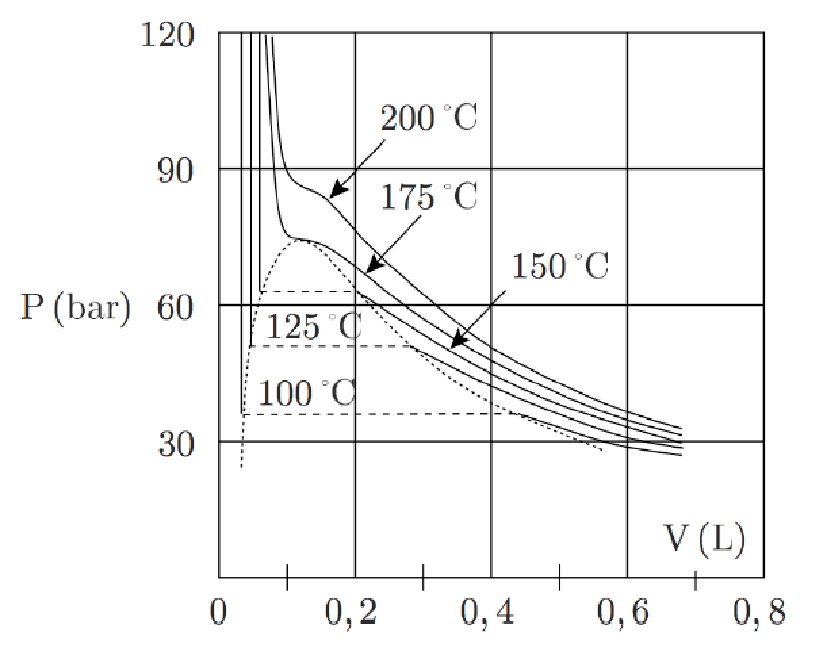
\includegraphics[scale=1]{iso_and}
    \label{fig:isoand}
  \end{center}
\end{minipage}

\section{Calorimétries}
\begin{rdefi}{Données}
  % \vspace*{-10pt}
  $c_{\rm eau} = \SI{4185}{J.K^{-1}.kg^{-1}}$ et $\Delta{h_{\rm fus}} =
  \SI{335}{kJ.kg^{-1}}$.
  % \vspace*{-10pt}
\end{rdefi}

\begin{multicols}{2}
  \subsection{Première expérience}
  Dans un calorimètre parfaitement isolé de capacité thermique $C =
  \SI{150}{J.K^{-1}}$, on place $m = \SI{100}{g}$ d'eau à la température $\theta
  = \SI{18}{\degreeCelsius}$ en équilibre thermique avec le vase intérieur et
  une masse $m_g = \SI{25}{g}$ de glace sèche à \SI{0}{\degreeCelsius}. Calculer
  la température d'équilibre.

  \subsection{Seconde expérience}
  Dans un calorimètre parfaitement isolé de capacité thermique $C =
  \SI{246}{J.K^{-1}}$, on place $m = \SI{100}{g}$ d'eau à la température $\theta
  = \SI{18}{\degreeCelsius}$ en équilibre thermique avec le vase intérieur et
  une masse $m_g = \SI{50}{g}$ de glace sèche à \SI{0}{\degreeCelsius}.
  Déterminer la température d'équilibre. Quelle proportion de glace a fondu~?
\end{multicols}

\section{Stockage d'eau chaude}
Une masse $m = \SI{100}{\kilo\gram}$ d’eau chaude est stockée dans une cuve
fermée de volume $V_0 = \SI{200}{L}$, que l’on modélise comme étant
indéformable. Pour simplifier, on ne tient pas compte de l’air contenu dans la
cuve en plus de l’eau. Suite à un échauffement accidentel, l’eau normalement
maintenue à $T_0 = \SI{60}{\degreeCelsius}$ passe à $T =
\SI{500}{\degreeCelsius}$.

La vapeur d’eau est modélisée par un gaz parfait. On tient compte de la légère compressibilité et dilatabilité de l’eau liquide par une équation d’état de la forme :
	\[
		\ln \frac{V}{V_0}=\alpha (T-T_0)-\chi_T(P-P_0)
		\qquad \text{avec} \qquad
		\left\{
		\begin{aligned}
			\alpha &= \SI{3.0e-4}{K^{-1}}\\
			\chi_T &= \SI{5.0e-10}{Pa^{-1}}
		\end{aligned}
		\right.
  \]
	
  \begin{figure}[h!]
    \centering
    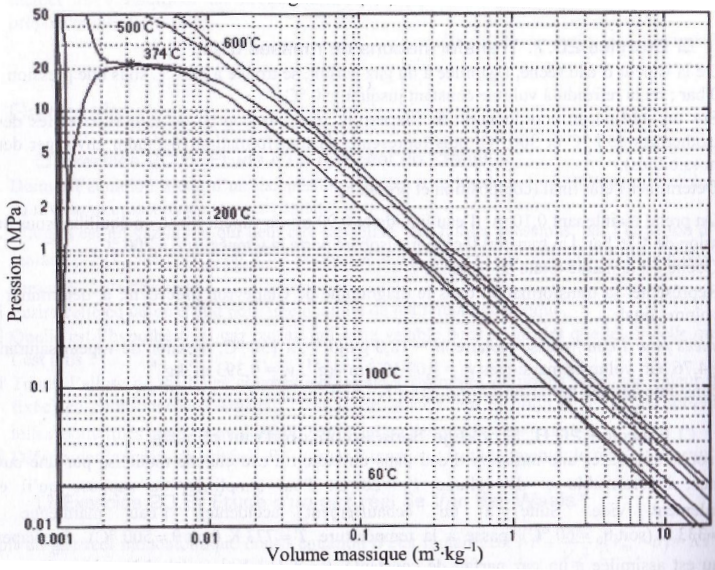
\includegraphics[width=.50\linewidth]{stock_eau}
    \caption{Diagramme de \textsc{Clapeyron} $(P,v)$ de l'eau. Plusieurs
      isothermes sont représentées pour des températures allant de 60 à
      \SI{600}{\degreeCelsius}. Attention, les échelles sont logarithmiques.
    }
    \label{fig:stock_eau}
  \end{figure}

\begin{enumerate}
  \item Identifiez, sur le diagramme de \textsc{Clapeyron}, la courbe de rosée,
  la courbe d'ébullition, le point critique et les différentes phases dans
lesquelles se trouve l'eau.

  \item Montrez que pour un équilibre liquide-vapeur, on a :
	\[
		x_g = \frac{m_g}{m_g+m_l} = \frac{v-v_l}{v_g - v_l}
  \]
  où $m_g$ représente la masse d'eau sous la forme "vapeur", $m_l$, la masse
  d'eau sous forme de liquide, $v$, le volume massique du mélange, $v_g$ et
  $v_l$, les volumes massiques des phases vapeur et liquide.

  \item En utilisant le diagramme de \textsc{Clapeyron}, déterminer la
    composition du mélange liquide-gaz initial.

  \item Sous quelle forme trouve-t-on l'eau après l'échauffement accidentel ?
  Déterminer la pression $P$ correspondante. Commenter.

  \item La soupape de sécurité permet au fur et à mesure du chauffage de laisser
    de la vapeur d’eau s’échapper~: la cuve est finalement presque vide et ne
    contient plus que $m_0 = \SI{400}{g}$ d’eau. Déterminer la pression
    finale et conclure.
\end{enumerate}

\section{Cycle de \textsc{Rankine}}
Un moteur fonctionne avec une masse $m$ d'eau. Cette masse d'eau subit les
transformations suivantes~:
\begin{itemize}
  \item AB~: isotherme (A liquide saturant à $T_1$ et $P_1$~; B à $P_2$)~;
  \item BC~: échauffement réversible isobare qui amène l'eau à la température
    $T_2$ (C liquide saturant)~;
  \item CD~: vaporisation totale sous la pression $P_2$ et à la température
    $T_2$~;
  \item DE~: détente adiabatique réversible jusqu'à la température $T_1$~;
  \item EA~: liquéfaction totale à la température $T_1$.
\end{itemize}
La capacité thermique massique de l'eau liquide vaut $c_{\rm liq} =
\SI{4.18}{kJ.K^{-1}.kg^{-1}}$. Dans le tableau suivant, on donne les
caractéristiques des points se trouvant sur la courbe de saturation aux pressions
$P_1$ et $P_2$.
\begin{table}[h!]
  \label{tab:rankine}
  \begin{center}
    \begin{tabular}{
        c
        S[table-format=1.3]
        S[table-format=3.2]
        S[table-format=1.2e1]
        S[table-format=1.3]
        S[table-format=3.2]
        S[table-format=4.1]}
      \toprule
      &
      {$P$ (\si{bar})} &
      {$T$ (\si{K})} &
      {$v_l$ (\si{m^3.kg^{-1}})} &
      {$v_g$ (\si{m^3.kg^{-1}})} &
      {$h_l$ (\si{kJ.kg^{-1}})} &
      {$h_g$ (\si{kJ.kg^{-1}})}

      \\\midrule
      {$P_1$} &
      0.250 & 338.15 & 1.02e-3 & 6.202 & 272.02 & 2618.4
      \\
      {$P_2$} &
      1.208 & 378.15 & 1.05e-3 & 1.419 & 440.17 & 2683.7
      \\
      \bottomrule
    \end{tabular}
  \end{center}
\end{table}

La variation d'entropie massique d'un liquide pour une transformation d'une
température $T_A$ à une température $T_B$ s'exprime
\[
  \Delta{s_{AB}} = s_{B} - s_{A} = c_{\rm liq}\ln \left(
  \frac{T_B}{T_A} \right)
\]
La variation d'entropie massique lors d'un changement d'état est~:
\[
  \Delta{s} = \frac{\Delta{h}}{T}
\]
avec $\Delta{h}$ la variation d'enthalpie massique lors du changement d'état et
$T$ la température du changement d'état.

\begin{enumerate}
  \item Tracer l'allure de deux isothermes d'\textsc{Andrews} dans le diagramme
    de \textsc{Clapeyron}. On fera apparaître la courbe de saturation. Dessiner
    l'allure du cycle sur ce même diagramme.
  \item 
    \begin{enumerate}
      \item Montrer que la variation $s_B - s_A$ est nulle.
      \item Exprimer $s_C - s_B$ en fonction de $c_{\rm liq}$, $T_1$ et $T_2$.
      \item Exprimer $s_D - s_C$ en fonction de $h_g(T_2)$, $h_l(T_2)$ et $T_2$.
      \item Calculer $s_E - s_D$.
    \end{enumerate}
  \item Énoncer le théorème des moments.
  \item Soit $x$ la fraction massique de vapeur en E. On admet que l'on peut
    appliquer le théorème des moments pour l'entropie. Déterminer $x$
    littéralement puis numériquement.
  \item Calculer les transferts thermiques massiques échangés lors des
    transformations BCD et EA.
  \item Déterminer le rendement du cycle. Application numérique.
\end{enumerate}

\section{Résolution de problème~: coca-cola}
Par une chaude journée d'été, vous avez oublié de mettre votre soda au frais.
Combien de glaçons faut-il ajouter pour que sa température descende à
\SI{5}{\degreeCelsius}~?

\end{document}
